\documentclass[]{IEEEtran}
% some very useful LaTeX packages include:
%\usepackage{cite}      
\usepackage{graphicx}   
\usepackage{subfigure} 
\usepackage{url}       
\usepackage{amsmath}    
\usepackage{caption2}
% Your document starts here!
\begin{document}

% Define document title and author
	\title{Weekly Report}
	\author{Adviser: Prof. Yang Wen \\Student: Cheng Wensheng\\ Period: 2018.8.20-8.26
	}
	\markboth{Visual Information Processing Group}{}
	\maketitle

% Write abstract here
\begin{abstract}
	This week I mainly put my effort on improving deep learning methods accuracy of building extraction with post processing.
\end{abstract}

% Each section begins with a \section{title} command
\section{Sar contest}
	% \PARstart{}{} creates a tall first letter for this first paragraph
	\PARstart{F}{rom} the result last week, we basicly use up the potential ability of semantic segmentation networks. So we tried to analyze the outcome of neural networks, and do some refinement works this week.	
	\begin{itemize}
		\item From the neural network output images, we can see that there are some black holes, surrounded by white buildings. Basically, there shouldn't be holes inside buildings. To fill these holes, we firstly find all contours in the image, which is the boundry of building, then fill these contours with white pixels. Finally, these holes were removed.
		\item Another problem is that there are some noises in the image. So we get rid of these noises by limiting the size of white area, since noise is generally small.
		\item We submitted this code, and the result shows about 0.5$\%$ improvement. This is not obvious.
		\item We are trying to seek for other methods to refine neural networks output image better to make use of the last chance.
	\end{itemize}
	
	Fig.~\ref{fig:fw} is RefineNet neural network result. Fig.~\ref{fig:rt} is GCN neural network result. Fig.~\ref{fig:imfill} is the post processing result of RefineNet model. Fig.~\ref{fig:gt} is the ground truth image.
	

% Main Part


\newpage


\begin{figure}
	\vspace{2.5cm}
	\begin{minipage}[t]{0.5\linewidth}
		\centering
		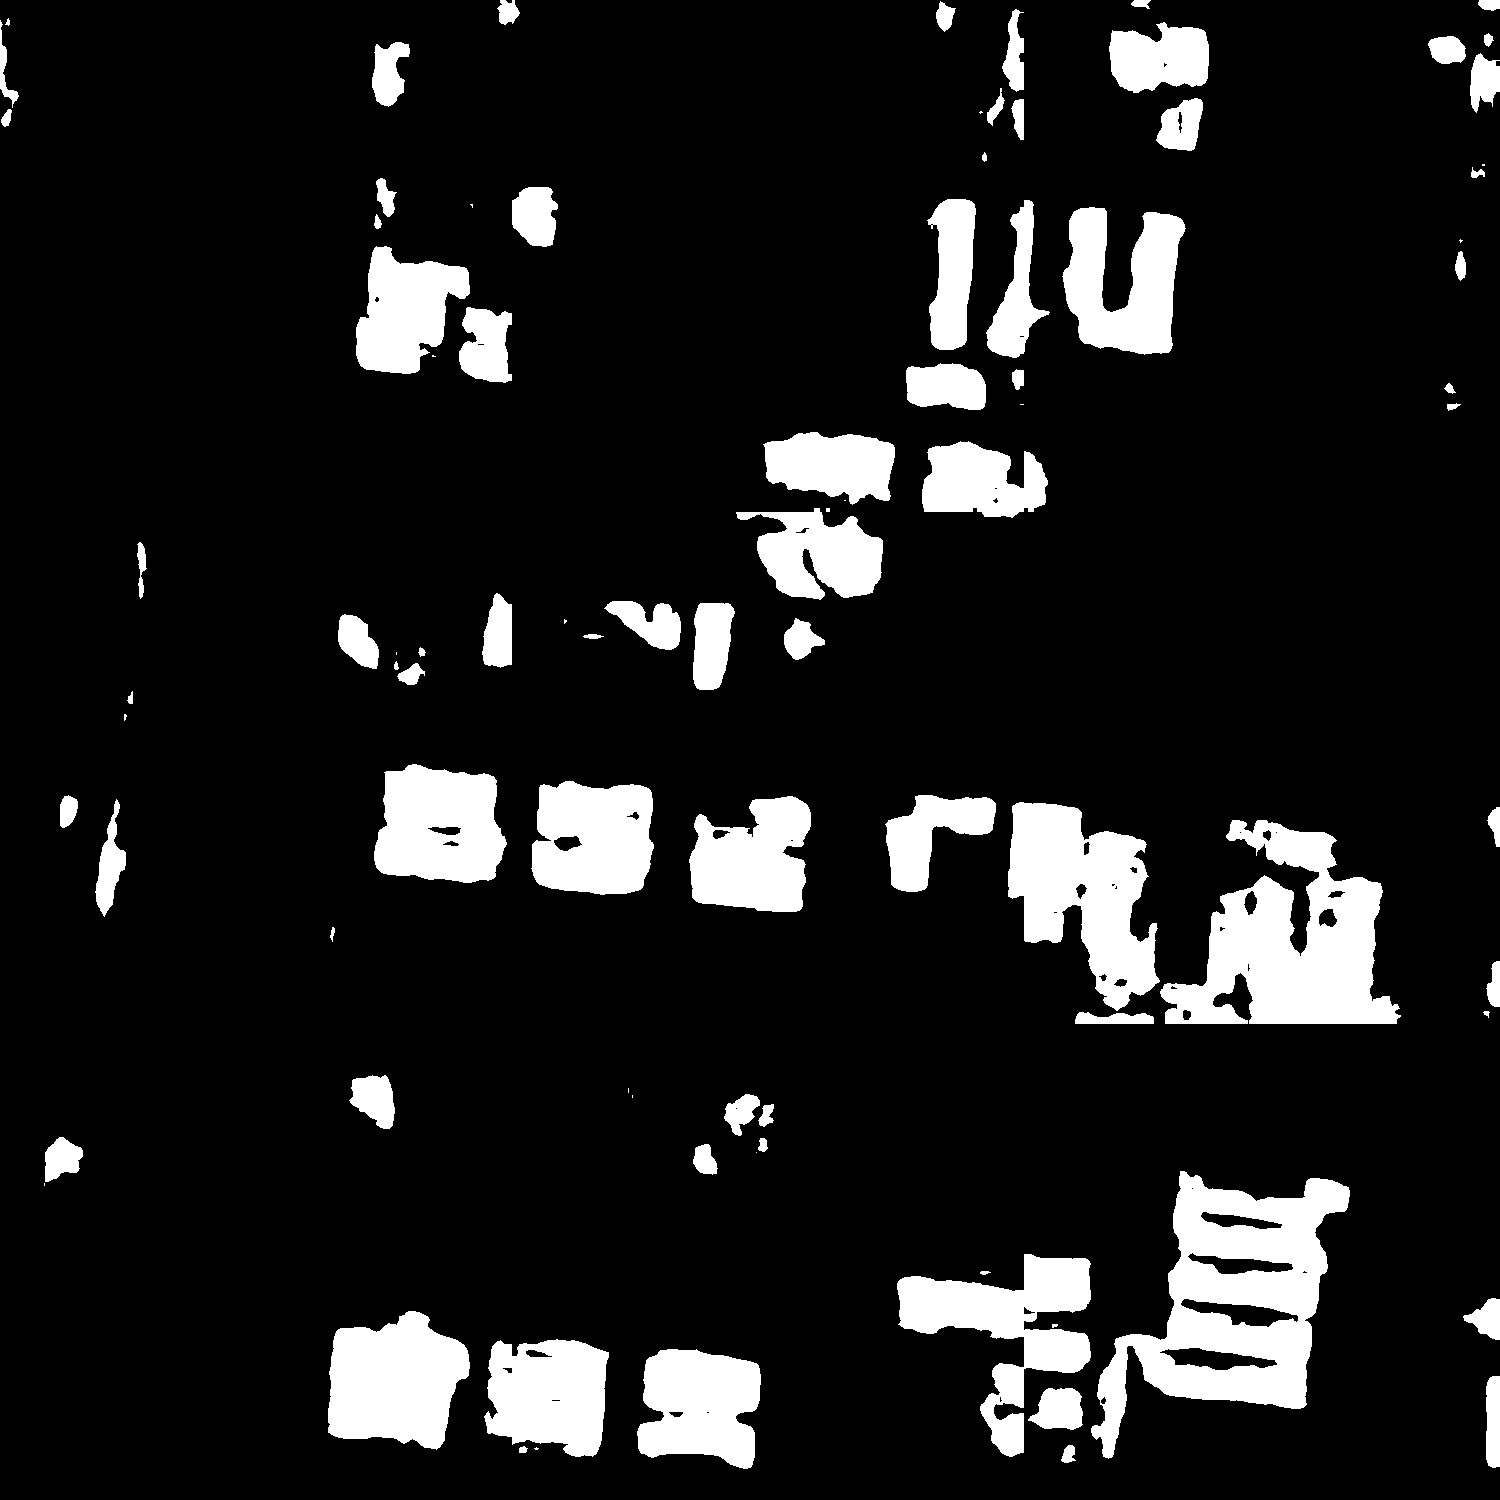
\includegraphics[width=0.9\columnwidth]{fw}
		\caption{RefineNet result}
		\label{fig:fw}
	\end{minipage}%
	\begin{minipage}[t]{0.5\linewidth}
		\centering
		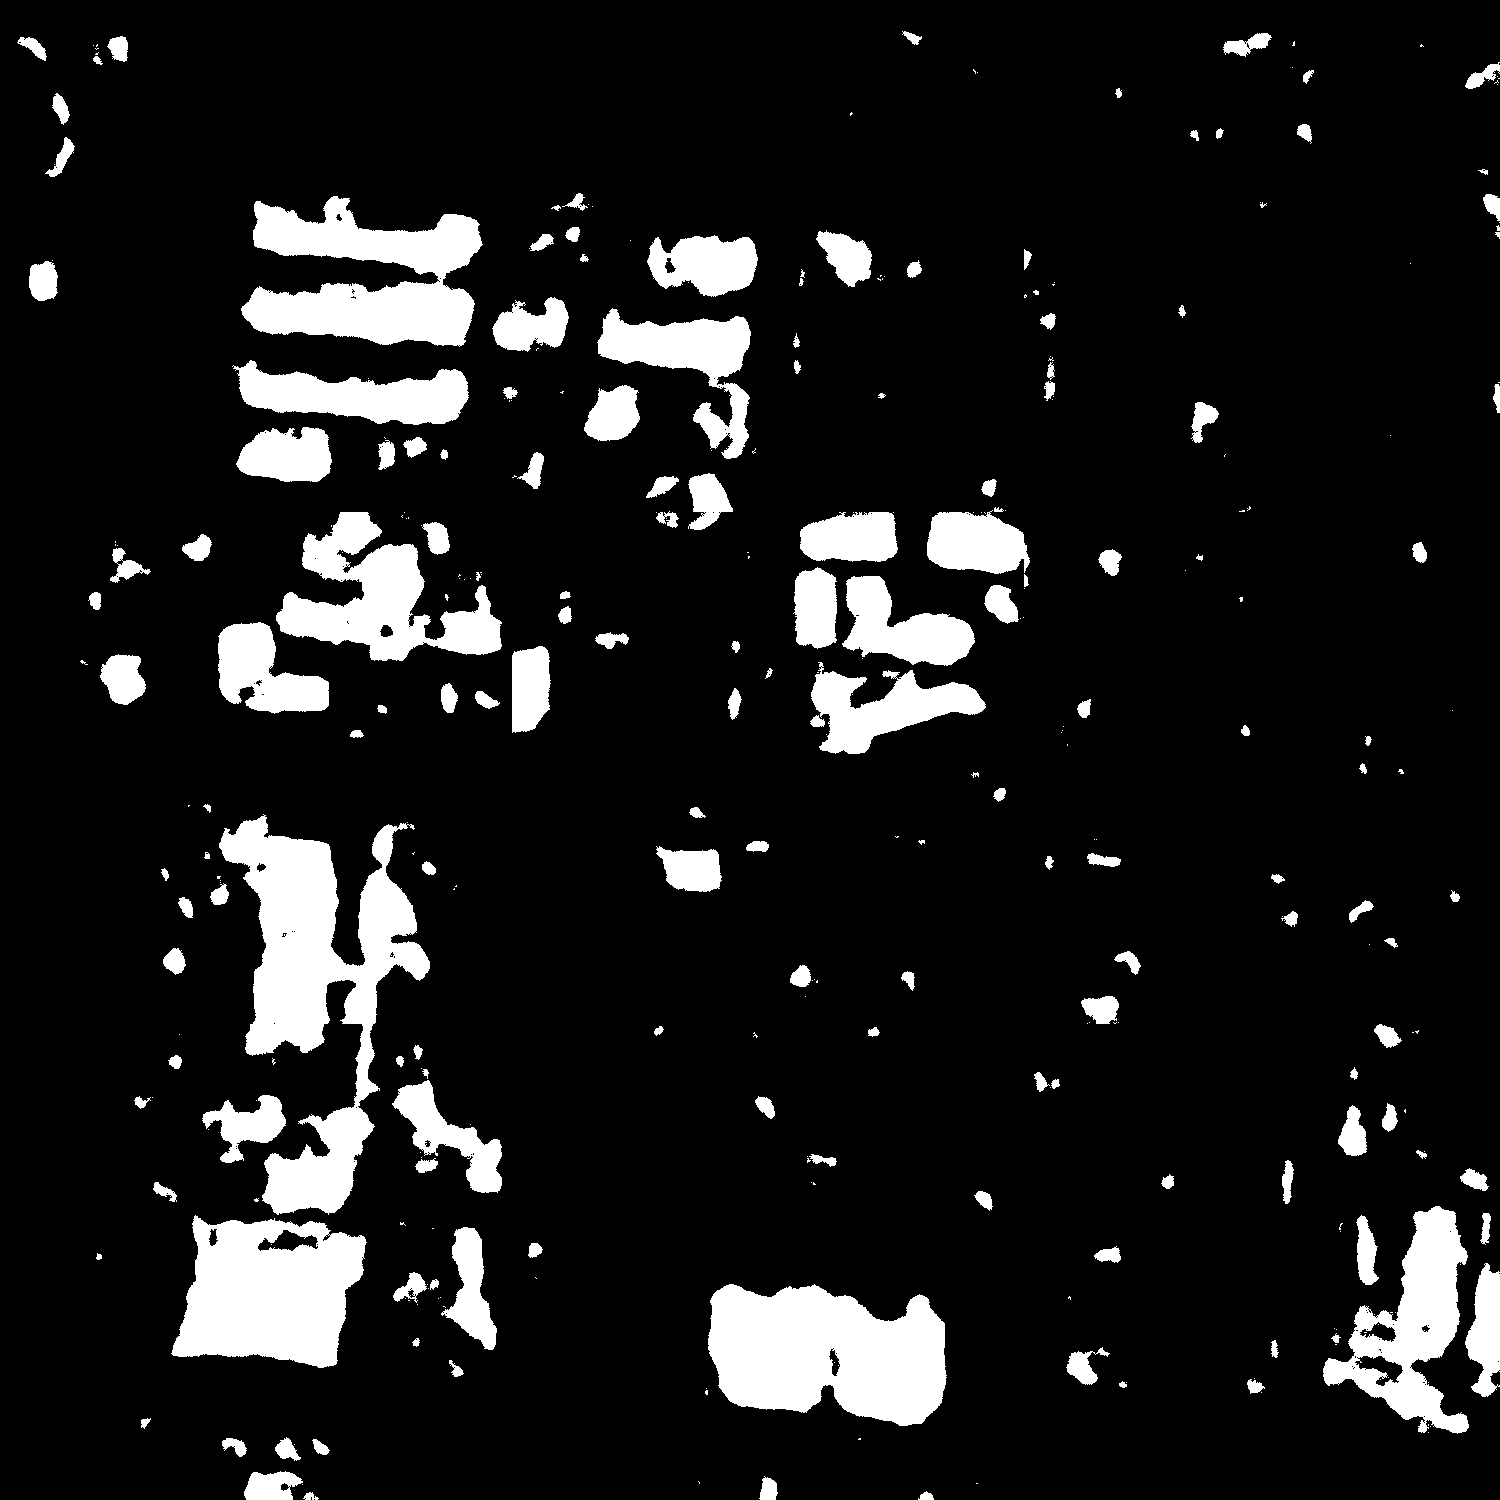
\includegraphics[width=0.9\columnwidth]{gcn}
		\caption{GCN result}
		\label{fig:rt}
	\end{minipage}
\end{figure}

\begin{figure}
%	\vspace{2.5cm}
	\begin{minipage}[t]{0.5\linewidth}
		\centering
		\includegraphics[width=0.9\columnwidth]{imfill}
		\caption{Post processing result}
		\label{fig:imfill}
	\end{minipage}%
	\begin{minipage}[t]{0.5\linewidth}
		\centering
		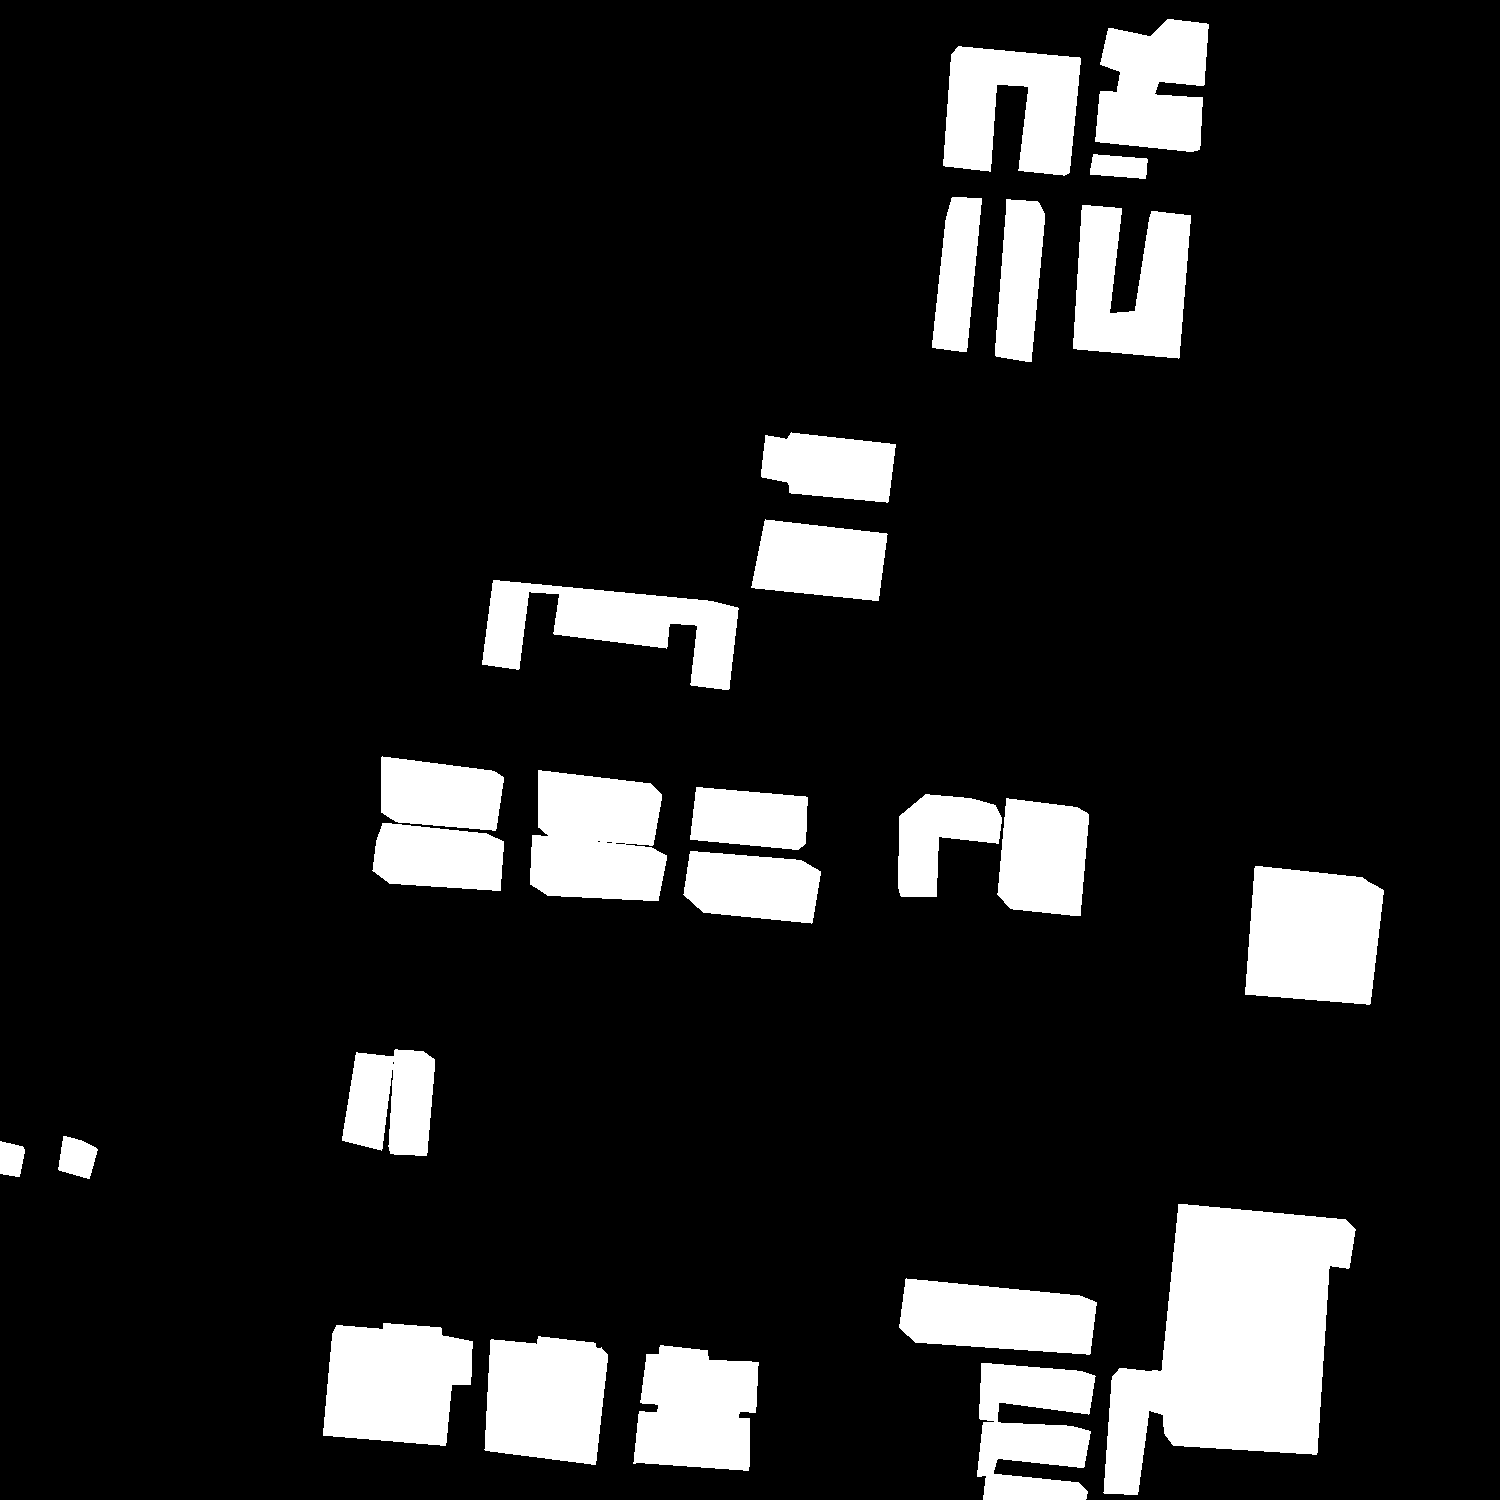
\includegraphics[width=0.9\columnwidth]{rs}
		\caption{Ground truth}
		\label{fig:gt}
	\end{minipage}
\end{figure}

%\begin{figure}[!hbt]
%%		 Center the figure.
%		\vspace{0.7cm}
%%		\hspace{50cm}
%		\begin{center}
%			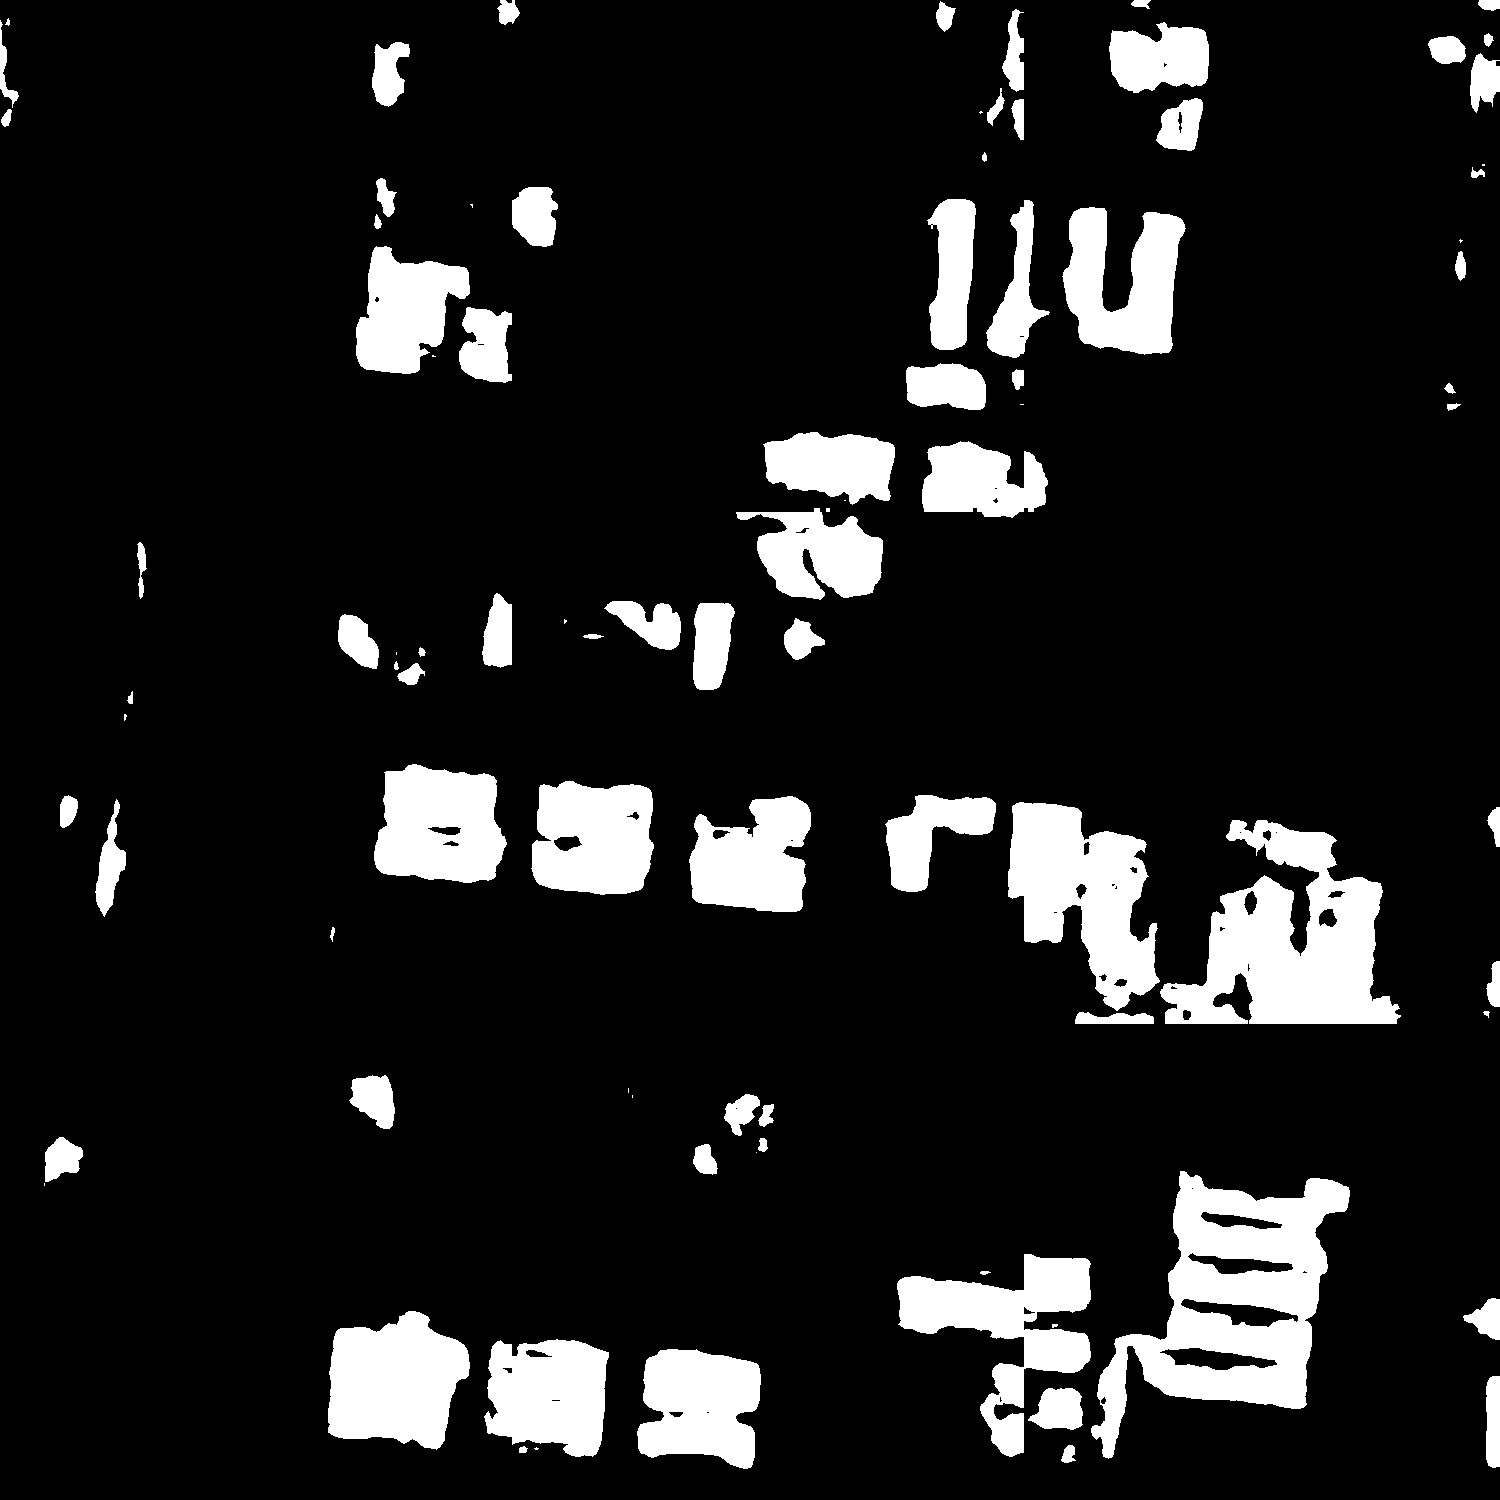
\includegraphics[width=0.2\columnwidth]{fw}
%				%		 Create a subtitle for the figure.
%			\caption{CNN methods result}
%			\label{fig:fw}
%		    \vspace{0.2cm}
%			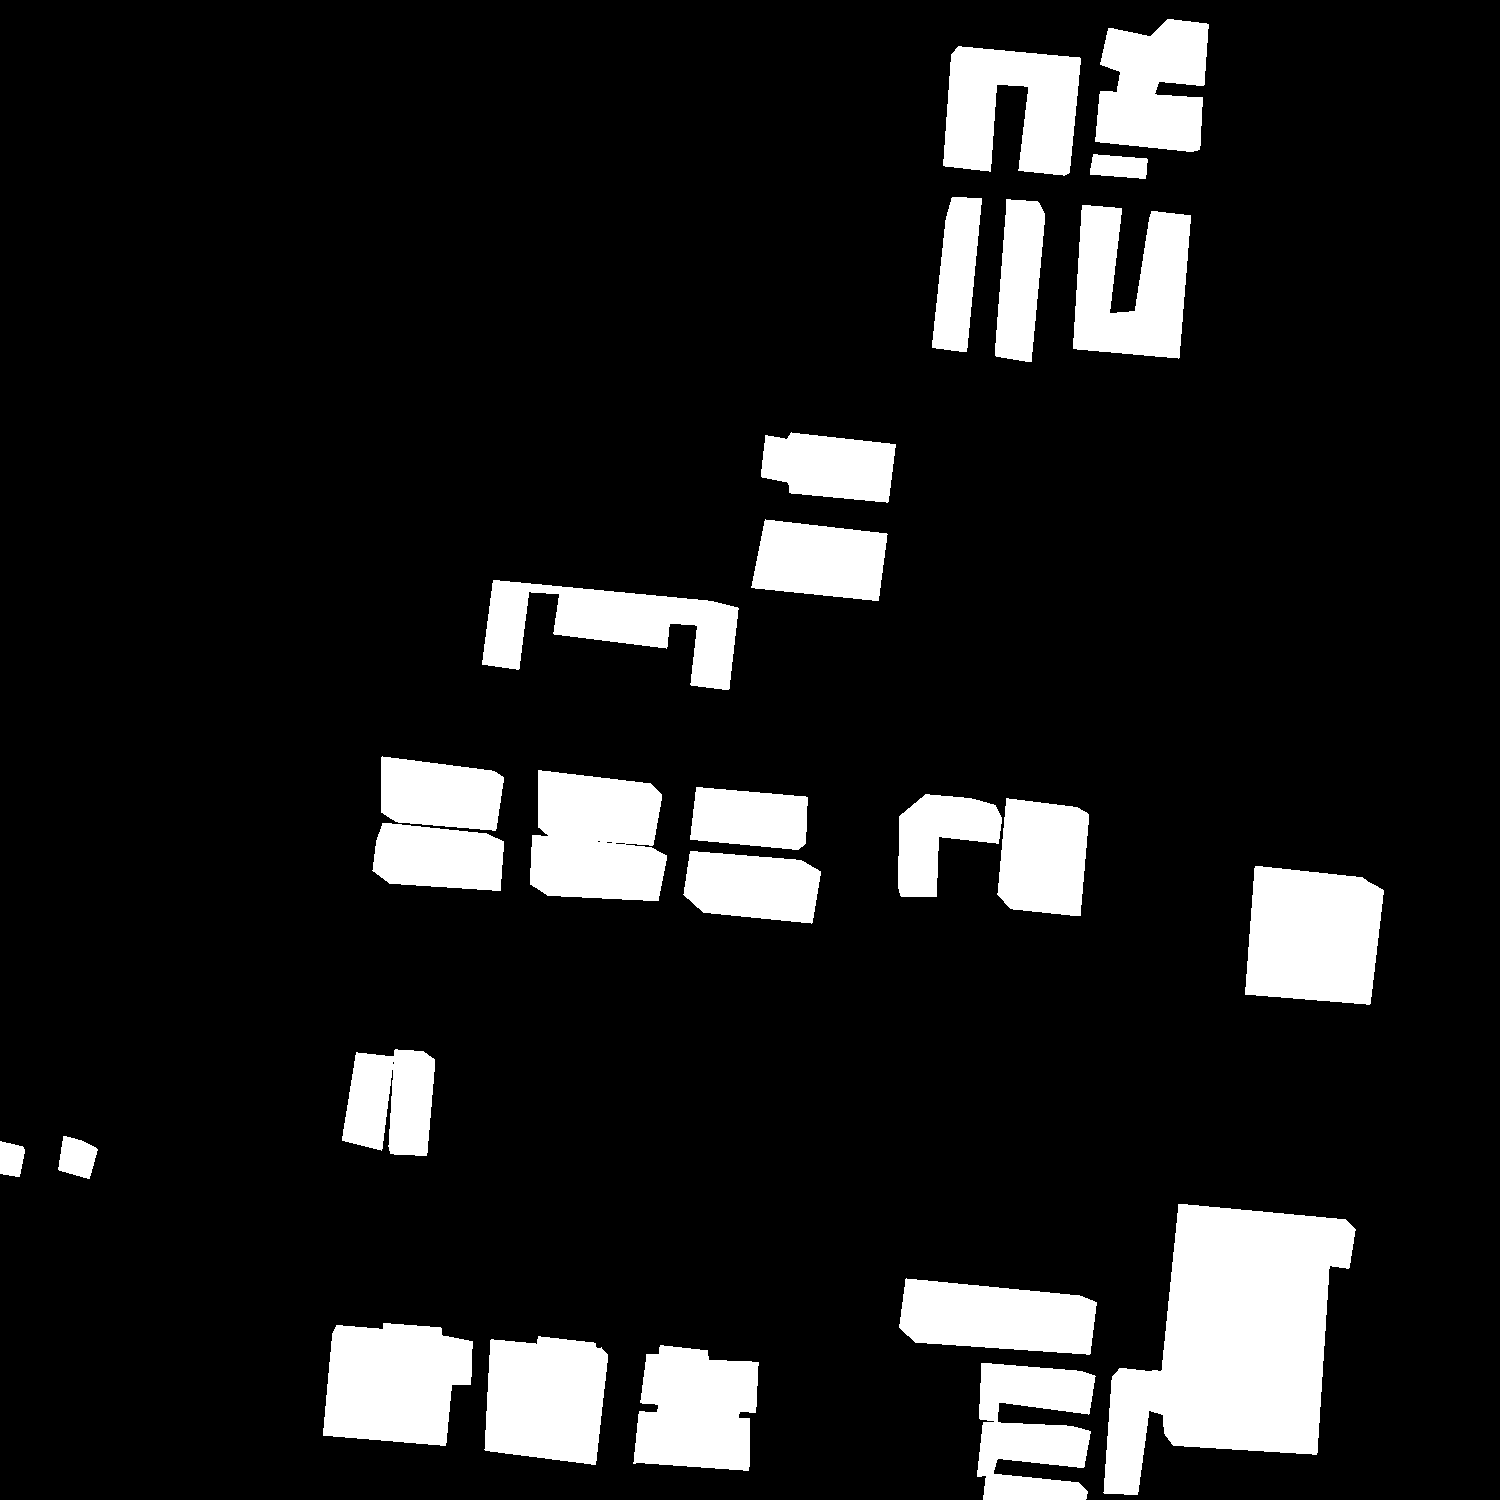
\includegraphics[width=0.2\columnwidth]{rs}
%				%Create a subtitle for the figure.
%			\caption{Ground truth}
%			\label{fig:rt}
%		\end{center}
%	\end{figure}



% Your document ends here!
\end{document}